\section{Vantaggi di Redpanda}
\subsection{Performance}
Redpanda è scritto in C++ e utilizza il \textit{framework} Seastar, offrendo un'architettura \textit{thread-per-core} ad alte prestazioni.
Ciò permette di ottenere un'elevata \textit{throughput} e latenze costantemente basse, evitando cambi di contesto e blocchi.
Inoltre, è progettato per sfruttare l'\textit{hardware} moderno, tra cui unità NVMe, processori \textit{multi-core} e interfacce di rete ad alta velocità.

\subsection{Costi}
Anche per carichi di lavoro ridotti, l'utilizzo di Apache Kafka può essere fino a 3 volte più costoso rispetto a Redpanda. Per carichi di lavoro più complessi, questa differenza può aumentare fino a 5 volte o più (\href{https://redpanda.com/blog/is-redpanda-better-than-kafka-tco-comparison}{fonte dei dati}).

\subsection{Semplicità di configurazione}
Il binario di Redpanda include, oltre al \textit{message broker}, anche un \textit{proxy} HTTP e uno \textit{schema registry}.

\subsection{BYOC (\textit{Bring Your Own Cluster})}
Redpanda offre una terza opzione oltre alla gestione autonoma di un \textit{cluster} di \textit{streaming}
dati e all'utilizzo di un servizio \textit{cloud} completamente gestito: \textit{Bring Your Own Cluster} (BYOC).
Questa alternativa consente agli utenti finali di implementare una soluzione parzialmente gestita dal fornitore nella propria infrastruttura (come il proprio \textit{data center}
o il proprio \textit{VPC cloud}).

\subsection{Compatibilità con API di Kafka}
Redpanda è progettato per essere compatibile con le API di Kafka, consentendo di utilizzare i \textit{client} Kafka esistenti senza modifiche.

\subsection{\textit{Self-healing}}
Redpanda è self-healing e redistribuisce continuamente i dati e la \textit{leadership} tra i nodi per mantenere il \textit{cluster} in uno stato ottimale mentre evolve o quando i nodi falliscono.


\begin{center}
	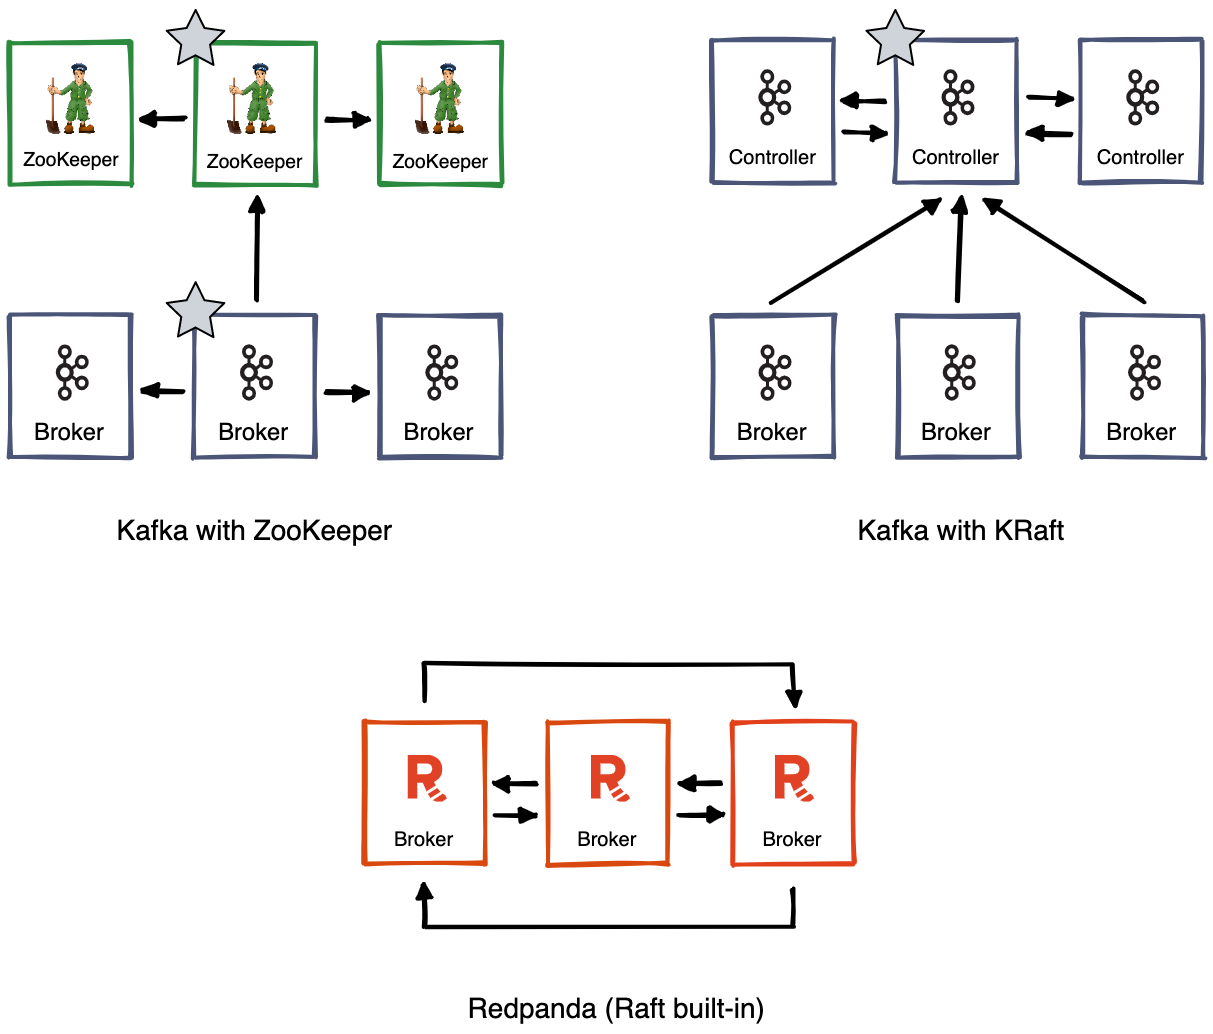
\includegraphics[width=0.65\textwidth]{imgs/kafka_zookeeper.png}
	\captionof{figure}{\href{https://redpanda.com/blog/kafka-kraft-vs-redpanda-performance-2023}{Architettura di Kafka con ZooKeeper}}
\end{center}












